%
% Qucs Test Report: SPICE to Qucs conversion: Test File 2
%
% Copyright (C) 2007 Mike Brinson <mbrin72043@yahoo.co.uk>
%
% Permission is granted to copy, distribute and/or modify this document
% under the terms of the GNU Free Documentation License, Version 1.1
% or any later version published by the Free Software Foundation.
%

% redefine subfigure caption
\renewcommand{\thesubfigure}{\thefigure(\alph{subfigure})}
\makeatletter
  \renewcommand{\@thesubfigure}{\thesubfigure:\space}
  \renewcommand{\p@subfigure}{}
\makeatother

% redefine subtable caption
\renewcommand{\thesubtable}{\thetable(\alph{subtable})}
\makeatletter
  \renewcommand{\@thesubtable}{\thesubtable:\space}
  \renewcommand{\p@subtable}{}
\makeatother

\tutsection{Introduction}
\tutsubsection{Title}
DC and independent voltage sin generator test.

\tutsubsection{SPICE specification}

Format:
\linebreak 
\bigskip 
\begin{footnotesize}\textbf{VX N+ N- [[DC]  DC/TRAN VALUE]  [AC [ACMAG [ACPHASE] ] ]}                                                          \end{footnotesize}
\linebreak 
Notes: 
\begin{enumerate}
 \item Characters [ and ] enclose optional items 
 \item Character / denotes OR
 \item Independent voltage source names begin with the letter V
 \item X denotes name of source
 \item N+ and N- are the positive and negative nodes respectively
 \item Voltage sources need not be grounded
\end{enumerate}

\begin{flushleft}
Specification of SPICE statement being tested:                                              \end{flushleft}


\textbf{VX N+ N- [[DC] VALUE] [SIN(VO VA [ FREQ [ TD [ KD ] ] ] ]}


\bigskip 


Notes:
\begin{enumerate}
 \item SIN generates a periodic sinusoidal signal, where
 \item VO is the DC offset; default: must be specified
 \item VA is the signal amplitude; default: must be specified
 \item FREQ is the signal frequency; default: value = 1/TSTOP
 \item TD is initial delay before sinusoidal signal starts; default: value = 0 seconds
 \item KD is the damping coefficient; default: value = 0. The damping factor has dimension 1/time.

\end{enumerate}




\tutsection{Test code and schematic}

SPICE code: File \verb|S2Q_test2.cir|

\begin{lstlisting}[
 language=Clean, 
 basicstyle=\small]

* SPICE to Qucs syntax test file 2
* DC and independent voltage sin sources, plus resistors.
*
.subckt S2Q_test2 p01 p02 p03 p04 p05 p06 p07 p08 p09 p10 p11
v1 p01 0 1v
r1 p01 0 10k
*
v2 p02 0 dc 1v
r2 p02 0 10k
*
*v3 p03 0 sin(0 5)
r3 p03 0 10k
*
v4 p04 0 sin( 0 5 1k)
r4 p04 0 10k
*
v5 p05 0 sin(0 5 1k 0.5m)
r5 p05 0 10k
*
v6 p06 0 sin(0 5 1k 0.5m 100)
r6 p06 0 10k
*
v7 p07 0 sin(0 5 1k 0.5m 1000)
r7 p07 0 10k
*
v8 p08 0 dc 5v sin(0 5 1k 0.5m 1000)
r8 p08 0 10k
*
v9 p09 0 sin(-5 5 1k 0.5m 1000)
r9 p09 0 10k
*
v10 p10 0 sin(5 5 1k 0.5m 1000)
r10 p10 0 10k
*
v11 p11 0 dc -10 sin(5 5 1k 0.5m 1000)
r11 p11 0 10k
.ends
.end


\end{lstlisting}


\begin{figure}
  \centering
  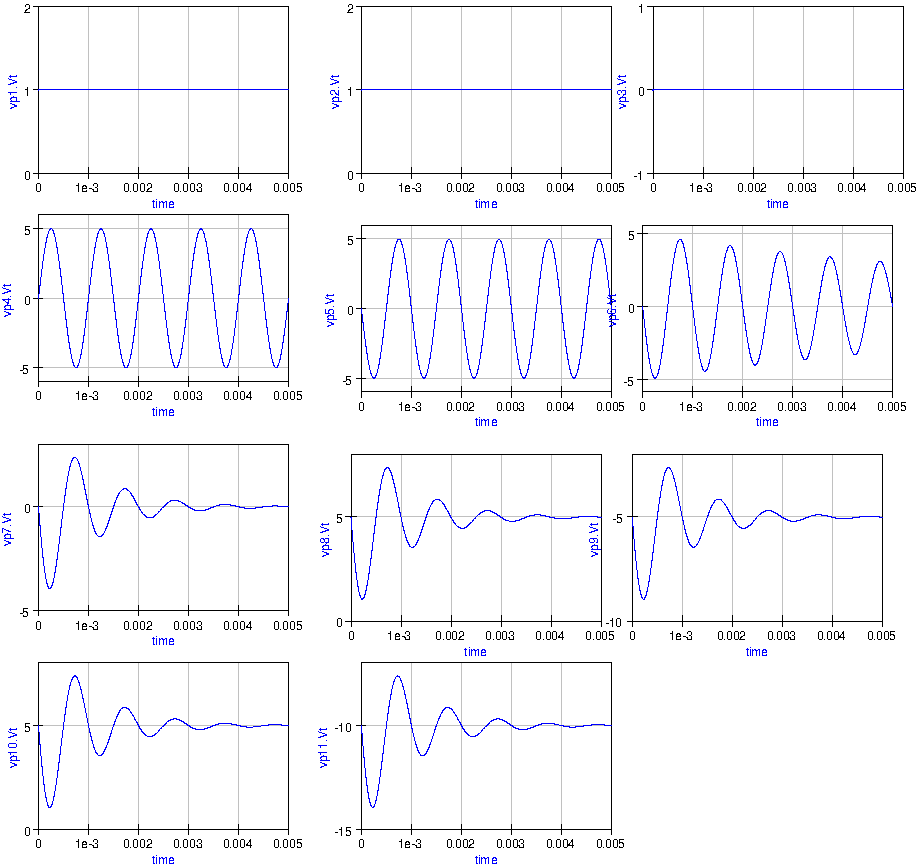
\includegraphics[width=0.8\linewidth]{S2Q_test2_sch}
  \caption{March 11: SPICE to Qucs conversion: Test2 waveforms}
  \label{fig:S2Qtest2_1}
\end{figure} 

\tutsection{History of simulation results}
\tutsubsection{March 11 2007, Simulation tests by Mike Brinson}
\begin{enumerate}
 \item Test 1  : Vp1.Vt;  Pass correct result.
 \item Test 2  : Vp2.Vt;  Pass correct result.
 \item Test 3  : Vp3.Vt;  \textbf{Fail} ERROR: line 17: checker error, no such variable `nan' used in a `Vac:V3' property  NOTE error occurs when v3 uncommented.
 \item Test 4  : Vp4.Vt;  Pass
 \item Test 5  : Vp5.Vt;  \textbf{Fail} TD should be 0.5m seconds - otherwise OK.
 \item Test 6  : Vp6.Vt;  \textbf{Fail} TD should be 0.5m seconds - otherwise OK.
 \item Test 7  : Vp7.Vt;  \textbf{Fail} TD should be 0.5m seconds - otherwise OK.
 \item Test 8  : Vp8.Vt;  \textbf{Fail} TD should be 0.5m seconds - otherwise OK
 \item Test 9  : Vp9.Vt;  \textbf{Fail} TD should be 0.5m seconds - otherwise OK
 \item Test 10 : Vp10.Vt;  \textbf{Fail} TD should be 0.5m seconds - otherwise OK
 \item Test 11 : Vp11.Vt;  \textbf{Fail} TD should be 0.5m seconds, plus DC level wrong.
\end{enumerate}




\begin{figure} 
  \centering
\begin{lstlisting}[
 language=Clean, 
 basicstyle=\scriptsize]
# Qucs 0.0.11  /media/hda2/S2Q_test2_prj/S2Q(test2).sch

.Def:S2Q_test2 _net0 _net1 _net2 _net3 _net4 _net5 
_net6 _net7 _net8 _net9 _net10
Sub:X1 _net0 _net1 _net2 _net3 _net4 _net5 _net6 
_net7 _net8 _net9 _net10 gnd Type="S2Q_test2_cir"
.Def:End

.Def:S2Q_test2_cir _netP01 _netP02 _netP03 _netP04 _netP05 
_netP06 _netP07 _netP08 _netP09 _netP10 _netP11 _ref
  .Def:S2Q_TEST2 _ref _netP01 _netP02 _netP03 _netP04 _netP05 
_netP06 _netP07 _netP08 _netP09 _netP10 _netP11
  Vac:V11 _netP11 _cnet8 U="5" f="1k" Phase="-180" Theta="1"
  Vac:V10 _netP10 _cnet7 U="5" f="1k" Phase="-180" Theta="1"
  Vac:V9 _netP09 _cnet6 U="5" f="1k" Phase="-180" Theta="1"
  Vac:V8 _netP08 _cnet5 U="5" f="1k" Phase="-180" Theta="1"
  Vac:V7 _netP07 _cnet4 U="5" f="1k" Phase="-180" Theta="1"
  Vac:V6 _netP06 _cnet3 U="5" f="1k" Phase="-180" Theta="0.1"
  Vac:V5 _netP05 _cnet2 U="5" f="1k" Phase="-180" Theta="0"
  Vac:V4 _netP04 _cnet1 U="5" f="1k" Phase="-0" Theta="0"
  Vac:V3 _netP03 _cnet0 U="5" Phase="-0" Theta="nan" f="1e+09" 
  Vdc:V1 _netP01 _ref U="1V"
  R:R1 _netP01 _ref R="10k"
  Vdc:V2 _netP02 _ref U="1V"
  R:R2 _netP02 _ref R="10k"
  Vdc:V3 _cnet0 _ref U="0" 
  R:R3 _netP03 _ref R="10k"
  Vdc:V4 _cnet1 _ref U="0"
  R:R4 _netP04 _ref R="10k"
  Vdc:V5 _cnet2 _ref U="0"
  R:R5 _netP05 _ref R="10k"
  Vdc:V6 _cnet3 _ref U="0"
  R:R6 _netP06 _ref R="10k"
  Vdc:V7 _cnet4 _ref U="0"
  R:R7 _netP07 _ref R="10k"
  Vdc:V8 _cnet5 _ref U="5V"
  R:R8 _netP08 _ref R="10k"
  Vdc:V9 _cnet6 _ref U="-5"
  R:R9 _netP09 _ref R="10k"
  Vdc:V10 _cnet7 _ref U="5"
  R:R10 _netP10 _ref R="10k"
  Vdc:V11 _cnet8 _ref U="-10"
  R:R11 _netP11 _ref R="10k"
  .Def:End
  Sub:X1 _ref _netP01 _netP02 _netP03 _netP04 _netP05 _netP06 
_netP07 _netP08 _netP09 _netP10 _netP11 Type="S2Q_TEST2"
.Def:End


.DC:DC1 Temp="26.85" reltol="0.001" abstol="1 pA" vntol="1 uV" 
saveOPs="no" MaxIter="150" saveAll="no" convHelper="none" Solver="CroutLU"
.TR:TR1 Type="lin" Start="0" Stop="5 ms" Points="2000" 
IntegrationMethod="Gear" Order="6" InitialStep="1 ns" MinStep="1e-16" 
MaxIter="150" reltol="0.001" abstol="100 pA" vntol="100 uV" Temp="26.85" 
LTEreltol="1e-3" LTEabstol="1e-6" LTEfactor="1" Solver="CroutLU" 
relaxTSR="no" initialDC="yes" MaxStep="0"
Sub:SUB1 vp1 vp2 vp3 vp4 vp5 vp6 vp7 vp8 vp9 vp10 vp11 Type="S2Q_test2"
\end{lstlisting}
 \caption{March 11: Qucs netlist showing V3 error [Edited to fit on page width]}
  \label{fig:S2Qtest2_2}
\end{figure} 



\begin{figure}
  \centering
  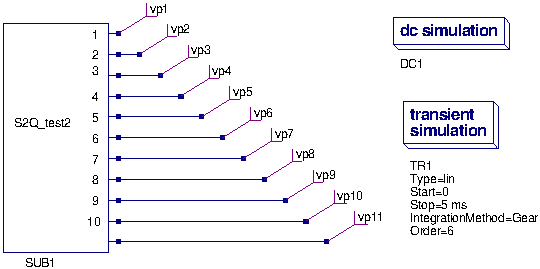
\includegraphics[width=0.9\linewidth]{S2Q_test2}
  \caption{SPICE to Qucs conversion: Test2 simulation schematic}
  \label{fig:S2Qtest2_3} 
\end{figure} 

\tutsubsection{March 12 2007, Simulation tests by Mike Brinson}
Code modifications: 
\begin{enumerate}
 \item * \verb|check_spice.cpp|: Fixed DC offset of sinuasoidal voltage and
        current sources.  Also apply default frequency if a transient
        analysis is given. Stefan Jahn
\item * vac.cpp, iac.cpp: Adjusted time dependency of damping
        factor Stefan Jahn
\end{enumerate}

\begin{enumerate}
 \item Test 1  : Vp1.Vt;  Pass correct result.
 \item Test 2  : Vp2.Vt;  Pass correct result.
 \item Test 3  : Vp3.Vt;  Pass - see note 1 below.
 \item Test 4  : Vp4.Vt;  Pass.
 \item Test 5  : Vp5.Vt;  Pass - see note 2 below.
 \item Test 6  : Vp6.Vt;  Pass - see note 2 below.
 \item Test 7  : Vp7.Vt;  Pass - see note 2 below.
 \item Test 8  : Vp8.Vt;  Pass - see note 2 below.
 \item Test 9  : Vp9.Vt;  Pass - see note 2 below.
 \item Test 10 : Vp10.Vt; Pass - see note 2 below. 
 \item Test 11 : Vp11.Vt; Pass - see note 3 below. 
\end{enumerate}

\begin{enumerate}
 \item The SPICE SIN generator assumes that the frequency of the generated sinusoidal signal equals 1/TSTOP if not explicitly given.  Hence, in such cases a .TRAN statement must be present in the simulated SPICE netlist; if a .TRAN statement is not included  a default frequency of f = 1GHz is used.  Also, when setting the transient simulation parameters using a Qucs transient analysis icon turn off SPICE simulation in the Edit SPICE Properties dialog box, otherwise two transient simulations are undertaken by Qucs.
 \item SPICE parameter TD is treated differently by Qucs.  In SPICE TD is the time from 0 seconds before the sinusoidal signal starts, causing the sinusoid to be non-linear.  In Qucs TD is implemented as a phase shift of a linear sinusoidal signal.  In the test example TD is 0.5m seconds which at f = 1kHz gives a phase shift of 180\degree  and is clearly visible in the test results. An error will probably occur if TD is greater than one signal period, 1m second in the test example.
\item Changes in CVS code have resulted in correct DC levels. 
\end{enumerate}




\begin{figure}
  \centering
  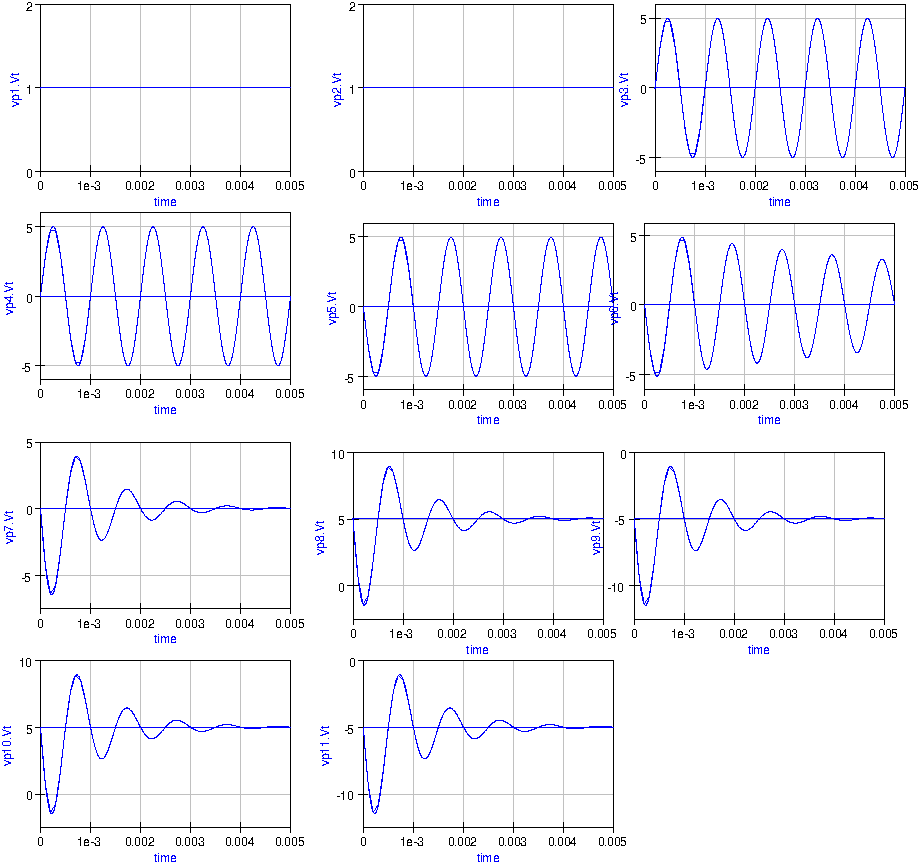
\includegraphics[width=0.8\linewidth]{S2Q_test2_M11}
  \caption{March 12: SPICE to Qucs conversion: Test2 waveforms}
  \label{fig:S2Qtest2_4}
\end{figure} 

\begin{figure} 
  \centering
\begin{lstlisting}[
 language=Clean, 
 basicstyle=\scriptsize]
# Qucs 0.0.11  /media/hda2/S2Q_test2_prj/S2Q(test2).sch

.Def:S2Q_test2 _net0 _net1 _net2 _net3 _net4 _net5 _net6 
_net7 _net8 _net9 _net10
Sub:X1 _net0 _net1 _net2 _net3 _net4 _net5 _net6 _net7
 _net8 _net9 _net10 gnd Type="S2Q_test2_cir"
.Def:End

.Def:S2Q_test2_cir _netP01 _netP02 _netP03 _netP04 _netP05 
_netP06 _netP07 _netP08 _netP09 _netP10 _netP11 _ref
  .Def:S2Q_TEST2 _ref _netP01 _netP02 _netP03 _netP04 _netP05
 _netP06 _netP07 _netP08 _netP09 _netP10 _netP11
  Vac:V11 _netP11 _cnet8 U="5" f="1k" Phase="-180" Theta="1"
  Vac:V10 _netP10 _cnet7 U="5" f="1k" Phase="-180" Theta="1"
  Vac:V9 _netP09 _cnet6 U="5" f="1k" Phase="-180" Theta="1"
  Vac:V8 _netP08 _cnet5 U="5" f="1k" Phase="-180" Theta="1"
  Vac:V7 _netP07 _cnet4 U="5" f="1k" Phase="-180" Theta="1"
  Vac:V6 _netP06 _cnet3 U="5" f="1k" Phase="-180" Theta="0.1"
  Vac:V5 _netP05 _cnet2 U="5" f="1k" Phase="-180" Theta="0"
  Vac:V4 _netP04 _cnet1 U="5" f="1k" Phase="-0" Theta="0"
  Vac:V3 _netP03 _cnet0 U="5" Phase="-0" Theta="0" f="1000"
  Vdc:V1 _netP01 _ref U="1V"
  R:R1 _netP01 _ref R="10k"
  Vdc:V2 _netP02 _ref U="1V"
  R:R2 _netP02 _ref R="10k"
  Vdc:V3 _cnet0 _ref U="0"
  R:R3 _netP03 _ref R="10k"
  Vdc:V4 _cnet1 _ref U="0"
  R:R4 _netP04 _ref R="10k"
  Vdc:V5 _cnet2 _ref U="0"
  R:R5 _netP05 _ref R="10k"
  Vdc:V6 _cnet3 _ref U="0"
  R:R6 _netP06 _ref R="10k"
  Vdc:V7 _cnet4 _ref U="0"
  R:R7 _netP07 _ref R="10k"
  Vdc:V8 _cnet5 _ref U="5"
  R:R8 _netP08 _ref R="10k"
  Vdc:V9 _cnet6 _ref U="-5"
  R:R9 _netP09 _ref R="10k"
  Vdc:V10 _cnet7 _ref U="5"
  R:R10 _netP10 _ref R="10k"
  Vdc:V11 _cnet8 _ref U="-5"
  R:R11 _netP11 _ref R="10k"
  .Def:End
  Sub:X1 _ref _netP01 _netP02 _netP03 _netP04 _netP05 _netP06
 _netP07 _netP08 _netP09 _netP10 _netP11 Type="S2Q_TEST2"
.Def:End

.TR:TRAN Points="11" Stop="1ms" Type="lin" Start="0"
.DC:DC1 Temp="26.85" reltol="0.001" abstol="1 pA" vntol="1 uV" 
saveOPs="no" MaxIter="150" saveAll="no" convHelper="none" Solver="CroutLU"
.TR:TR1 Type="lin" Start="0" Stop="5 ms" Points="2000" 
IntegrationMethod="Gear" Order="6" InitialStep="1 ns" MinStep="1e-16"
 MaxIter="150" reltol="0.001" abstol="100 pA" vntol="100 uV" Temp="26.85"
 LTEreltol="1e-3" LTEabstol="1e-6" LTEfactor="1" Solver="CroutLU" 
relaxTSR="no" initialDC="yes" MaxStep="0"
Sub:SUB1 vp1 vp2 vp3 vp4 vp5 vp6 vp7 vp8 vp9 vp10 vp11 Type="S2Q_test2"

\end{lstlisting}
 \caption{March 12: Qucs netlist showing V3 error [Edited to fit on page width]}
  \label{fig:S2Qtest2_2}
\end{figure} 


\tutsection{References}
\begin{enumerate}
 \item A. Vladimirescu, Kaihe Zhang, A.R. Newton, D.O Pederson A. Sangiovanni-Vincentelli, SPICE 2G User's Guide (10 Aug 1981), Department of Electrical Engineering and Computer Sciences, University of California, Berkeley, Ca., 94720.
\item B. Johnson, T. Quarles, A.R. Newton, P.O. Pederson, A.Sangiovanni-Vincentelli, SPICE3 Version 3f User's Manual (October 1972),  Department of Electrical Engineering and Computer Sciences, University of California, Berkeley, Ca., 94720.
\item Andrei Vladimirescu, THE SPICE book,1994, John Wiley and Sons. Inc., ISBN 0-471-609-26-9.
\end{enumerate}


